\documentclass[11pt,a4paper]{article}
\usepackage[show]{ed}
\usepackage{tikz}
\usepackage{float}
\usepackage{hyperref}
\usepackage[style=alphabetic, backend=bibtex]{biblatex}
\usepackage{graphicx}

\title{Building Mathhub using React\\ \vspace{2 mm} Bachelor Thesis}
\author{Johannes-Sebastian See\\Supervisor: Michael Kohlhase\\Co-supervisor: Tom Wiesing\\Friedrich-Alexander University, Erlangen Nürnberg, Germany}

\date{\today}
\addbibresource{local.bib}

\begin{document}

\begin{titlepage}
\maketitle
\begin{abstract}
Abstract will be added at the end
\end{abstract}

\end{titlepage}

\tableofcontents
\section{Introduction}
\subsection{Math Information Systems}
\ednote{why are those special and different}
\subsection{Mathhub}
\subsection{Previous Implementation}
Up until April 2018 the Mathhub frontend was realized with Drupal.
Drupal is an open source content-management framework used by millions of different websites.
Dealing with user interactions were handled by JavaScript modules in the JOBAD framework \cite{comp}.
	
But in April 2018 a critical security flaw in the versions 6 to 8 went public.
The problem was that the Drupal core in these versions accepts request parameters without any validation.
This means the core processes any input from anybody \cite{zdnet}.
To exploit this weakness an attacker doesn't even need to log in or have any other privileges on a vulnerable website \cite{register}.
With this flaw it is possible to inject malicious code and compromise a website in multiple ways.
This can be used to access, change and delete private data and create backdoors to make future attacks possible.
The Drupal community called this weakness "Drupalgeddon2" while its official name was "CVE-2018-7600".
Some code that was injected installed the program XMRig Monero miner, which is a cryptocurrency mining program, as well as deleting other mining programs on the compromised system \cite{hacker}.
The National Institute of Standards (NIST) and Technology gave Drupal a "Highly Critical" Rating because of this vulnerability \cite{nist}.
 After this flaw was discovered a patch was published and a warning to update every website that used a vulnerable version was given.
	
Since there have been multiple flaws in Drupal before that compromised Mathhub, the decision to stop using it and rebuild Mathhub from the ground up to not be affected by future attacks, was made.

\section{State of the art}
\subsection{Building an interactive Frontend}
Before starting to build a completely new Mathhub frontend a different web framework had to be chosen.

\textbf{Polymer} is an open source JavaScript library developed and maintained by Google.
It provides a set of features that make creating custom elements, that work like standard web components, easy.
It is used for several Google services for example Youtube, Google Earth, Google Play Music etc. as well as Netflix, Electronic Arts and many other companies. \cite{polymer}

Another open source web framework from Google is \textbf{Angular}.
This TypeScript library has framework architectures that simplifies the development of new web applications.
It also has Angular Material.
A collection of UI components that work in browsers, on mobile and desktop. \cite{angular}

After using Angular on several Google projects, Evan You decided to create his own JavaScript framework called \textbf{Vue.js} \cite{vuewiki}
Depending on the project it can be scaled between a framework and a library.
Vue.js separates its view layer library from its support libraries for complex applications, to create an easy approach to the framework. \cite{vuegit}

In the end the decision was made to use \textbf{React} developed by Facebook.
Further details about React and how it is used can be found in section \ref{preliminaries}.

\subsection{Math Information Systems}
\begin{itemize}
\item MathNet
\item mathoverflow
\item Wikidata
\item Wikipedia
\end{itemize}

\section{Preliminaries} \label{preliminaries}
\subsection{The core concept of React} 
React is an open source JavaScript library owned and maintained by Facebook.	It was created to build interactive user interfaces (UI).
For example it is used for Facebook and Instagram.
What makes React unique is its use of a virtual Document Object Model (DOM).
The concept of the virtual DOM is that when updating a website not everything is rendered again.
React computes the differences between the last and the next page and only changes the necessary parts.
On top of that it has conditional rendering which means that an item will only be rendered if it is shown.
The advantage of virtual and conditional rendering is that this makes updating a website fast, but it comes with high RAM costs.
The actual interface is made up of many different elements and components.
Since a website that uses React can have many different features it is helpful to build new components.
\cite{reactjs}
React does not have a styling system so it integrates Semantic UI to provide a consistent theme for the frontend.

\subsection{Building new components in React}
React already has a large library with a lot of different components, but it is often necessary to make new ones that have the desired functionality.
In JavaScript new components can be implemented by creating either a function or a class.
Their input variables are called props and can only be read.
Components return React elements that are ready to be rendered.
Naturally a component can grow big rather quickly.
Luckily it is possible to use components inside other components.
This comes with the advantage that they can be reused in many different locations.
The difference between creating a new component as a function and as a class is that a class can have a private internal state, which can be updated an any time.
Since props are read-only, updating the state can only affect lower components.
If it is necessary to also change something in a higher component it is possible to "lift up" the state.
This means adding the state that causes the change to the state of the component on a higher level and giving it back to the lower levels as a prop.
If the update should affect a component on the same level creating a new component with that state that consist of all the one that are affected will  make this possible.
\cite{reactjsGS}

\subsection{MMT and OMDoc}
\begin{itemize}
\item OMDoc: XML format of how a uniform language for knowledge should be designed
\item MMT is a scalable Module System for Mathematical theories
\item MMT is a framework for knowledge representation using formal languages
\item individual features are defined as reusable modules -> create individual languages
\item high degree of abstraction of advanced algorithms
\item archives: correspond to software projects; work flows for languages in MMT
\item groups / libraries: collection of archives
\item module: theory or view
\item view: relations between theories
\item theory: defined by declarations
\item declaration: constants and rules
\item groups and archives just for narration
\item modules and declarations are actual content
\cite{mmt}
\end{itemize}
 
\section{The Architecture of Mathhub}

\providecommand\myxscale{.95}
\providecommand\myyscale{1}

\subsection{Mathhub.info Routes}
\begin{figure}[h]
\begin{tikzpicture}[xscale=\myxscale, yscale=\myyscale]
  \tikzstyle{component} = [rectangle, draw, fill=blue!20, text width=2cm, text centered,
                                    rounded corners, minimum height=.8cm,shade, 
                                    top color=white, bottom color=blue!20]
\node[component] (MH) {Mathhub};
\node[component, below of =MH, xshift=-1.2cm, yshift=-0.7cm] (lib) {Library};
\node[component, below of =lib, yshift=-0.7cm] (groups) {Groups};
\node[component, below of =groups, yshift=-0.7cm] (archives) {Archives};
\node[component, below of =archives, text width=5cm, text height=1.8cm, yshift=-1.3cm, label ={[shift={(0ex,-4ex)}]north:Modules}] (mod) {};
\node[component, below left of =mod, xshift=-0.5cm, yshift=0.5cm] (theo) {Theories};
\node[component, below right of =mod, text width=1.5cm, xshift=0.5cm, yshift=0.5cm] (views) {Views};
\node[component, below of=mod, yshift=-1.2cm] (decl) {Declarations};
\node[component, below left of =MH, xshift = -4.3cm, yshift=-0.7cm] (apps) {Applications};
\node[component, below left of =apps, xshift=-0.5cm, yshift=-0.7cm] (glos) {Glossary};
\node[component, below right of =apps, xshift=0.5cm, yshift=-0.7cm] (dict) {Math Dictionary};
\node[component, below of=MH, xshift=1.6cm, yshift=-2.4cm] (news) {News};
\node[component, below of=MH, xshift=2.8cm, yshift=-1.4cm] (log) {Log};
\node[component, below right of=MH, xshift=3.7cm, yshift=-0.7cm] (legal) {Legal};
\draw[->,dotted] (MH) -- node[above]{} (lib);
\draw[->,dotted] (MH) -- node[above]{} (apps);
\draw[->,dotted] (MH) -- node[above]{} (news);
\draw[->,dotted] (MH) -- node[above]{} (log);
\draw[->,dotted] (MH) -- node[above]{} (legal);
\draw[->,thick] (lib) -- node[above]{} (groups);
\draw[->, thick] (groups) -- node[above]{} (archives);
\draw[->,thick] (archives) -- node[above]{} (mod);
\draw [->,thick] (mod) -- node[above]{} (decl);
\draw[->,thick] (apps) -- node[above]{} (glos);
\draw[->,thick] (apps) -- node[above]{} (dict);
\end{tikzpicture}
\caption{Mathhub components}
\end{figure}

To create a logical navigation system Mathhub.info is divided into numerous pages, that can be accessed from the Home-page.

First of is the main content of Mathhub, the MMT library.
It starts with the different groups.
The next page displays the archives that belong to a specific group.
Groups and archives only exists for narration and navigation purposes.
So they don't have any actual content only meta information like names and descriptions.
The actual content can be found in documents.
These document consist of several theories and views.
So the archive-page has a list of all the documents in an archive.
On the document-page the modules are displayed with all their declarations.


With the huge mathematical library of theories there are a lot of technical terms.
The glossary is a collection of these expressions.
There wouldn't be much value in to just having a collection without any additional features.
So the glossary also provides a definition for each term.
Over the time many different authors have contributed to the theories, so it can happen that there are different terms that share a meaning.
These synonyms can also be found in the glossary.
Since many theories exist in multiple languages it makes sense to have a glossary available for every used language.
Currently the biggest collection of terms are in the English glossary, followed by German and French.
Smaller collections for Turkish and Romanian are also available as well as simplified and traditional Chinese.

Most of the times a user does not want to browse through the gigantic glossary to just find a single term.
This is the reason why the Math Dictionary is a useful extension of the glossary.
The main purpose of the Math Dictionary is to translate a term into another language and look up a definition of a specific expression.


There is also a page with all the latest news regarding Mathhub, \ednote{or MMT? or KWARC?} as well as pages for licenses and the privacy policy.
At last there is a Log with the most recent messages from the backend. \ednote{is this right?}

\subsection{Layout}
Every page consists of three parts: A header, a footer and the actual content in between.

The header is a menu with the routes to Home, the news, the glossary and the Math Dictionary as well some external links.
Under the menu there are breadcrumbs for an easier navigation.
In the footer the logos of the institutions that are involved in Mathhub can be found.
There also are the routes to the Log, the licenses, the imprint and the privacy policy.
The body itself depends on the page the user is currently on.
\ednote{Screen shots}

\subsection{Realization}
\ednote{name pending}
\begin{figure}[H] \label{architecture}
\begin{tikzpicture}[xscale=\myxscale,yscale=\myyscale]
  \tikzstyle{system} = [rectangle, draw, fill=blue!20, text width=1cm, text centered,
                                    rounded corners, minimum height=.8cm,shade, 
                                    top color=white, bottom color=blue!20]
   \tikzstyle{database} = [rectangle, draw, fill=blue!20, text width=1cm, text centered,
                                    rounded corners, minimum height=.8cm,shade, 
                                    top color=white, bottom color=blue!20]
\node (user) {user}; 
\node[system,right of =user,text width=2cm, xshift=3cm] (browser) {Browser}; 
\node[system,right of= browser,text width=2.3cm, xshift=2.6cm] (drupal) {React};
\node[system,above right of =drupal, xshift = 2.8cm] (mmt) {MMT};
\node[system,below right of =drupal, xshift = 2.8cm, text width=1.2cm] (gl) {GitLab};
\node[database,below left of =gl, yshift = -0.6cm, xshift = -3cm] (lib) {library};
\node[below right of =gl, yshift = -0.6cm, xshift = 1.6cm] (author) {author}; 
\node[below right of =mmt, yshift =0.7cm,  xshift = 1.6cm] (conv) {\begin{tabular}{l}\footnotesize convert to\\ OMDoc\\/MMT\end{tabular}};
\draw[<-,thick] (mmt) -- node[left]{load} (gl);
\draw[<->,dotted] (user) -- node[above]{read} node[below]{interact} (browser);
\draw[->,thick] (browser) -- node[above]{REST} (drupal);
\draw[->,thick] (gl) to[loop left,out=20,in=45,looseness=11] (gl); 
\draw[<->,dashed] (conv) -- (mmt);
\draw[<-,thick] (drupal) -- node[above]{present}(mmt); 
\draw[->,thick] (drupal) -- node[above]{edit}(gl); 
\draw[->,dotted] (author) -- node[above]{local} node[below]{edit} (gl);
\draw[->,dotted] (lib) -- node[below]{import} (gl);
\end{tikzpicture}
\caption{Mathhub architecture}
\end{figure}
\ednote{look for author and user pictures}
\ednote{React doesn't edit anything yet, so maybe erase the edit-arrow?}

The React based frontend that is displayed in the browser is written in TypeScript.
The use of Semantic UI React achieves an informal theme throughout Mathhub.info.
The React frontend is in constant communication with an MMT server that provides the user with the actual content as well as several semantic services.


Whereas React is used for the presentation of the content documents, GitLab is used for their versioned storage.
There the documents are organized into their proper repositories and converted from the source format into the OMDoc/MMT format.
These documents can be edited in a working copy of the GIT repository.
Afterwards the author can submit the changes with a direct commit.

\subsection{Communication with the Backend}

As previously mentioned the frontend does not have any actual content.
It gets the data from the MMT backend.
The frontend has several clients that each communicate with the server when their specific functionality is needed.
The different clients are:
\begin{itemize}
\item a Library Client for everything related to the content of the library
\item a Glossary Client that gets all the terms in a specific language
\item a Translation Client that is used by the Math Dictionary to search for a translation of a term 
\item a News Client
\item a Log Client
\end{itemize}

The answers that are received from the backend use the JavaScript Object Notation (JSON).
The data objects in JSON consist of attribute-value pairs and arrays.
The frontend then uses these objects to build React components.


\section{Mathhub Library Components}
This chapter is about the implementation of the different components of the Mathhub library.
The first page of the library is a list of all the groups of Mathhub.
Every group is rendered in its own React component that has the name of the group, a short teaser and links to the corresponding group-page.

\subsection{Groups}
Above the numerous archives the group page starts with a header that has the same structure for every group.
It begins with a button that links to its source files on GitLab.
After that follows a description that gives an overview of the groups content.
The header ends with a list of e-mail addresses of the people that maintain the group.

Beneath that there is a list of all the corresponding archives.
Every archive is its own React component that consists of a name and a short teaser that summarizes its content for the user.
By clicking on an entry the user is taken to the corresponding archive-page.
\begin{figure}[H]
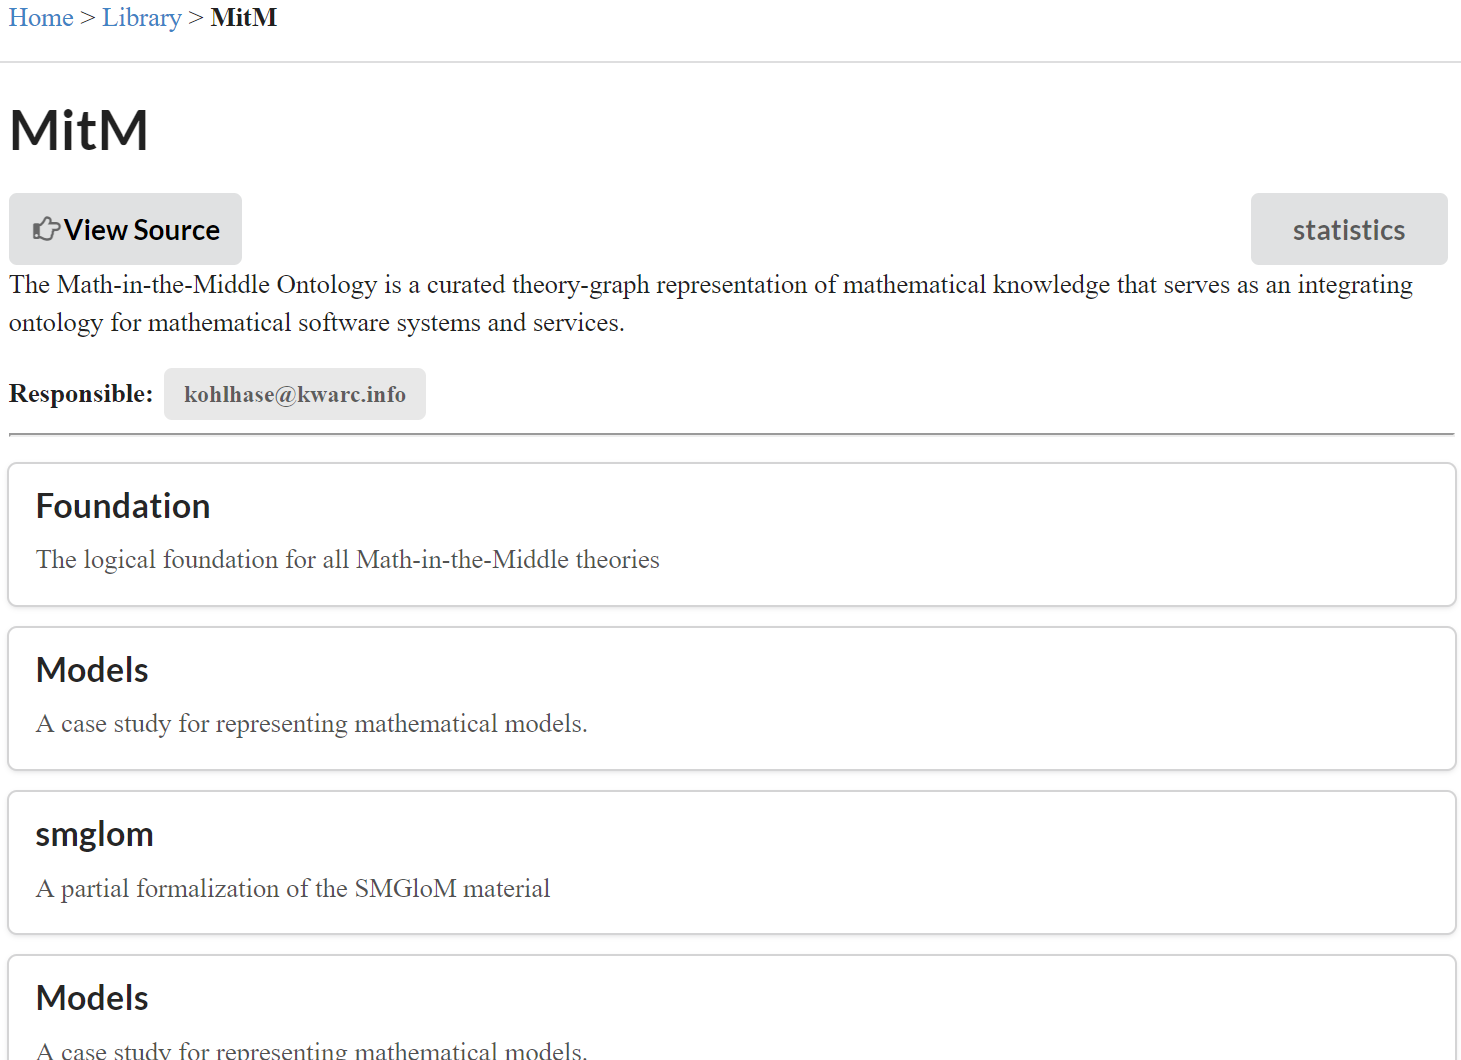
\includegraphics[width=1\textwidth]{group.png}
\caption{a group in the frontend}
\end{figure}

\subsection{Archives}
The structure of the archive-page is very similar to the group-page.
It also starts with a header that consists of a button that links to the source files, a description of the archive and the e-mail addresses of the responsible people.

After the header follows a list of the documents in that archive.
There is the main difference between the group-page and the archive page.
The document entries do not have a teaser text so they just link to the document-page.
\begin{figure}[H]
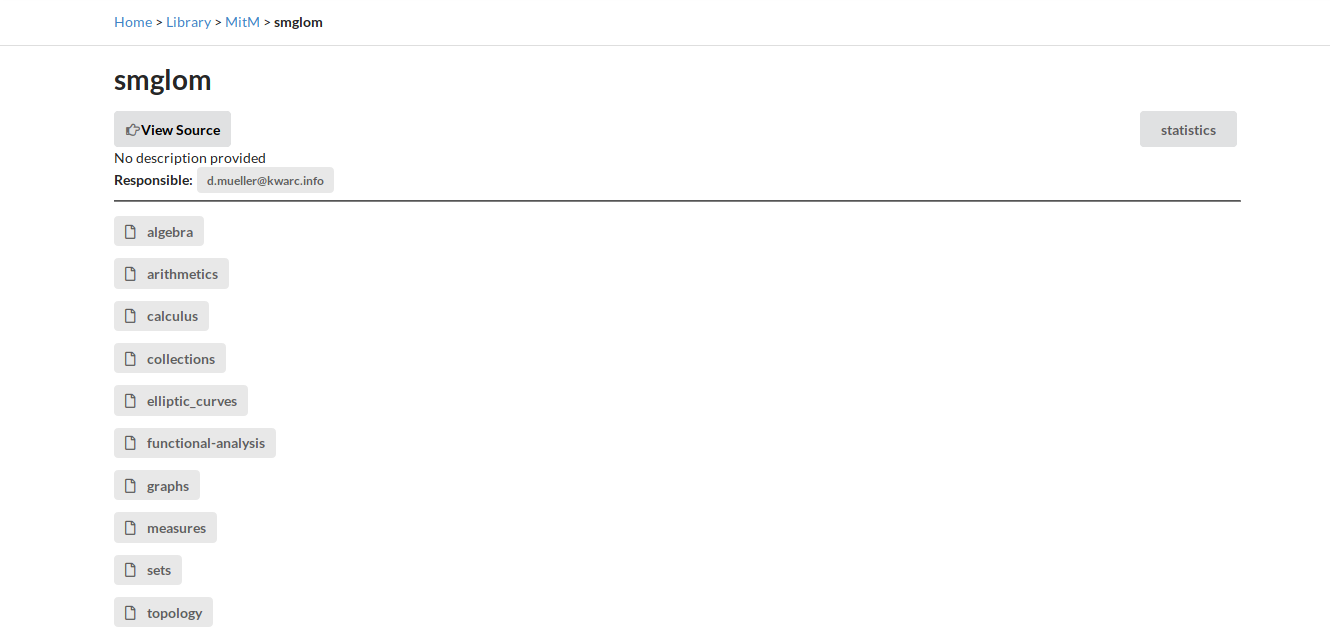
\includegraphics[width=1\textwidth]{archive.png}
\caption{ an archive in the frontend}
\end{figure}

\subsection{Documents}
Depending on the document the document-page can be either a list of OMDocs or the different modules of an OMDoc. \ednote{can i write it like this?}
If the document is in the OMDoc format there is also a button that links to its source file on GItLab.
The modules of a document are expandable React components that consist of a name, a type, either theory or view and a button to show further details.
Clicking on the button shows all the declarations and nested theories inside of a module.
These declarations (structure elements or constants) and theories can be further extended to show their own content.

In between the modules there can be opaque elements.
These are just text that help the user to understand the content of the document and do not serve any contribution to the actual theories
\begin{figure}[H]
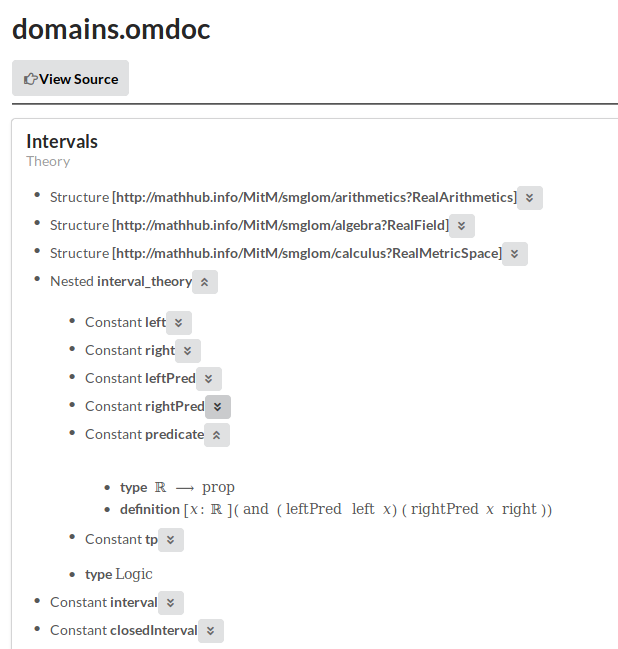
\includegraphics[width=1\textwidth]{document.png}
\caption{a document in the frontend}
\end{figure}

\subsection{Statistics}
On every group-, archive- and document-page there also is a statistics button that shows some available statistics about that particular group, archive or document.
When the cursor hovers over a keyword of a statistic that keyword is explained in a pop-up.
\begin{figure}[H]
\centerline{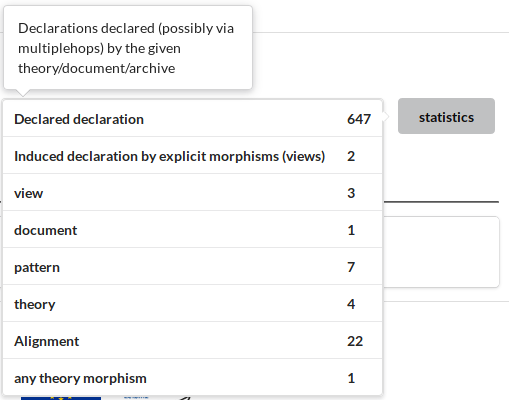
\includegraphics[width=0.6\textwidth]{statistics.png}}
\caption{statistics in the frontend}
\end{figure}

\section{The Applications of Mathhub}

\subsection{Glossary}
The glossary-page has a tab for every available glossary.
At any given time only the terms are rendered that have an entry in the currently selected language.
Thus it is possible to change languages by either changing the language tab or clicking on a language-button inside an entry.
If there is a button with a different language available, this means this particular entry also exists in that language.
To create a better overview the definition of a term is not immediately shown.
By clicking on an entry the definition becomes visible.
\begin{figure}[H]
\includegraphics[width=1\textwidth]{glossary.png}
\caption{the glossary in the frontend}
\end{figure}

\subsection{Math Dictionary}
To translate a term with the help of the Math Dictionary the user has to select the language from a dropdown menu in which the term currently is and also the language to which it should be translated into
Pressing the "translate" - button sends a translation request to the server.
Until the servers responds, the message "translating" is shown and the button is disabled to prevent sending to many translation requests.
If a translation exists then the translated term, its definition and potential synonyms are shown.
By selecting the same language for "from" and "to" the Math Dictionary can also be used to get the definition for an expression without searching the glossary.
\begin{figure}[H]
\includegraphics[width=1\textwidth]{dictionary.png}
\caption{the Math Dictionary in the frontend}
\end{figure}

\section{Conclusion}

\section{Future Work}
	\subsection{TGView}
	\subsection{MathWebSearch}
	\subsection{Subset Frontends}
	\subsection{Issue report: Mathhub and content}

\printbibliography
\ednote{use this: github.com/KWARC/bibs/kwarc.bib}
\end{document}